\chapter{Background}
	\section{Introduction}
		\subsection{The Problem}
			Intellectual Property law is a term typically used to describe the areas of law which establish property protection over intangibles such as ideas, signs and information. This protection is in order to make the advancement of ideas profitable which therefore incentivises this act\cite{ip_edu_bently}.
			
			There is, therefore, a balance to be struck between limited exclusive rights and benefits to the public. While limiting exclusive rights may facilitate progress, benefiting the public, the overprotection of the exclusive property may restrict their access\cite{handbook_ip_hr_geiger}. One example of this is the expansion of copyright terms such as the contreversial Copyright Term Extension Act of 1998 which was heavily lobbied for by Disney just years before Mickey Mouse's copyright ran out\cite{mickey_mouse_grzelak}. The trend in extension of copyright terms, illustrated by Figure \ref{fig:ext_us_cop}, illustrates the appearance that the balance is tipping towards exclusivity rights. 

			\begin{figure}[h]
    			\centering
    			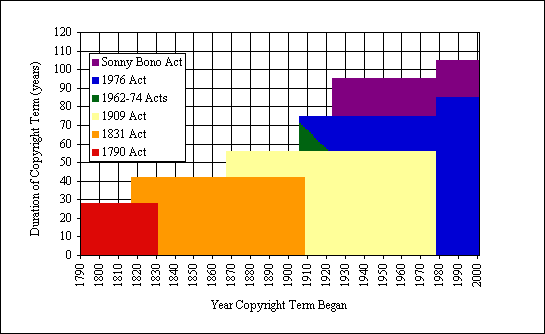
\includegraphics[width=0.5\linewidth]{resources/images/extention_of_us_copyright.png}
    			\caption{Expansion of U.S. copyright term lengths\cite{copyright_term_length_graph_bell}.}
    			\label{fig:ext_us_cop}
			\end{figure}
			
			This implementation of intellectual property law brings in the question of human rights of access to culture, education and other social and economic rights, but traditionally this has not been included in discussion of intellectual property law\cite{mapping_ip_hr_helfer}. However, recently scholarship and legislation has progrssively begun to incorporate each other's linguistics\cite{bileta_proposal_blakely}.
			
			Dr. Megan Rae Blakely of Lancaster University is looking for assistance in analysing journals and legal instruments for overlap in languages. In this analysis, I will map the dynamics of this change in legal and social perspective, to make evident moments of significant shifts in language. 
			
			Previously, analysis of the intersection between human rights and intellectual property law, such as Helfer's\cite{hr_ip_conflict_coexistence_helfer}, has been limited to more manual case-by-case methods. Supplying a more systematic method using natural language processing that can cope with large amounts of data would give concrete evidence of the relationship between human rights and intellectual proeprty. 
		\subsection{Aims and Objectives}
			In the early stages of the project, the following requirements for the project were established:
			\begin{itemize}
				\item A model that takes a corpus of training PDF documents as input and assess the typical language characteristics of intellectual property documents and human rights documents and which indicates the extent to which each document suggests the law protects the user or the creator/owner;
				\item A visualisation of this model with the $x$-axis as time; the $y$-axis as the intent of the document toward human rights to intellectual property; and the $z$-axis as the measure of the extent to which the document suggests the protection of the creator/owner or the user;
				\item An easy to use Graphical User Interface which allows for input of law journals and treaties in PDF form and then outputs the updated visualisation;
				\item A code base written and documented well enough for any future researcher to easily understand and extend on.
			\end{itemize}
			
			Over the course of the literature review, section \ref{sec:litrev}, I will review past literature in order to find the best methods to achieve each of these requirements.
		\subsection{Added Value}
			The originality of the project stems from its application of natural language processing methods in this domain, rather than the natural language processing methods used. The added value will be the unique way in which the findings are best illustrated for this application through the visualisation.
			
			The outcome of the project will help add value to its domain. As the first systematic, easily scalable technology in this domain, it will help illustrate how historical changes in technology have impacted the tone of intellectual law. Blakely points out that this, in turn, will allow legal professionals to consider how future technological changes will impact their work and adapt accordingly.
	\section{Literature Review} \label{sec:litrev}	
		\subsection{Machine Learning Classifiers} \label{sec:litrev:mlclass} % ADD EQUATIONS
			Document topic classification is the automated assignment of natural language texts to predefined categories based on their content\cite{ml_automated_categorisation}. 
			
			The precision/recall break-even point is a typical measure of success in topic classification\cite{encyc_breakeven_sammut}. It is obtained by modifying parameters until the precision and recall values are equal. However, this breakeven point does not always exist\cite{bigrams_enhance_categorisation}. An alternative to this is F1-score which is calculated by multiplying two by the precision and recall and then deviding this by the sum of the precision and recall. 
		
			Support vector machines are a common feature-based approach to classification. They work by considering words occuring in the training set (alternatively, see section \ref{sec:litrev:langfeat}) as a feature and plotting each document in the feature space by the number of times each feature occurs in it. It then plots a hyperplane that best splits each document class. This led to an 86\% precision/recall breakeven point when they classified the Reuters 'acq' dataset\cite{svm_joachims}. %ADVANTAGES AND DISADVANTAGES
			
			In contrast to support vector machines, Naive Bayes is a probabilistic approach based on Bayes' rule. Bayes' rule is a formula for finding the class given a document. There are many variations of this type of classification where the likelihood, representing the probability of a document given a class, differs. The Bernoulli multivariate model only considers whether a word occurs in a document while the multinomial model considers how many times a word appears in each document. Predictably, McCallum and Nigam found that the multinomial model performs consistently stronger over any significant vocabulary size. This led to a 89\% precision/recall breakeven point when classifying the Reuters 'acq' dataset, slightly better than Support Vector Machine's 86\%.%ADVANTAGES AND DISADVANTAGES COMPARED TO SVM

			Wang and Manning improved the performance of both naive Bayes and support vector machines, for datasets with average wordcounts over 100, by adding naive Bayes features to support vector machines\cite{baselines_bigrams_wang}. 
			
			All these methods assume that each document can only be a member of one class. This is often not the case. Godbole and Sarawagi use the example that if a document is classed as being about wheat, it is also likely to be about grain\cite{discriminative_multilabel_godbole}. This relationship between topics should be captured in a topic-topic distribution and took advantage of. Godbole and Sarawagi implement a few variations of this, all based around the standard support vector machines with one added feature per class representing how similar the given class is to all other classes. It leads to a slight improvement on F1-score across two datasets.
			
		\subsection{Language Features} \label{sec:litrev:langfeat}	
			The models from Section \ref{sec:litrev:mlclass} mostly used single words as features. This is known as a bag of words model. This has the benefit of having dense feature spaces and therefore, higher computational efficiency but it is not representative of the actual meaning of text. Wallach points out that the phrases "the department chair couches offers" has a vastly different topic to "the chair department offers couches", yet a bag of words model will represent them as the same\cite{beyond_bag_wallach}. This sort of ambiguity would clearly give innacurate results so it is worth using a feature a bit more resource heavy that provides more accuracy.
			
			The most common feature used is an n-gram model. This is where $n$ words are taken as the feature, giving each word some ordered context. Tan et al use bigrams that pass a certain threshold to avoid the feature space being too sparce, combined with unigrams resulting in a 3\% average F1-score improvement on the Reuters datasets\cite{bigrams_enhance_categorisation}.
		\subsection{Graphical Visualisation}
			What visualisations have been used for topic classification before?
			
			What visualisations have been used in the law domain before?
		\subsection{Iterative Process}
			HCI - how to review in an iterative process
		\subsection{User Interface}
			Nielsen collated his heuristics from existing sets of heuristics with the aim of creating a general set which is as good as possible at explaining the usability prblems hat occur in real systems\cite{usability_heuristics_nielsen}. These have been highly regarded since he finalised them in 1994. They are as follows: 
			\begin{itemize}
				\item The user must be kept informed of the system status;
				\item The system must match the real world with concepts familiar to the user;
				\item The user must have control over the system, especially with an easy emergency exit;
				\item The system should be consisent with its looks and actions;
				\item The system should do everything within its power to prevent errors;
				\item The system should make the user's options visible so they do not have to memorise them;
				\item The system should be flexible so novice users can use with ease but expert users can use hidden accelerators for more efficient use;
				\item The design should be aesthetic and minimalist since every piece of information is competing for the user's attention;
				\item The system should give error messages that are expressed in plain language, that precisely indicate the problem and that constructively suggest a solution;
				\item The system should provide help and documentation for the user in case anything about the system is unclear.
			\end{itemize}
			Nielsen also presents how to measure the severity of usability problems. The severity of a problem is split into three categories: the frequency with which a problem occurs which is how commonly it occurs; the impact of when it occurs which is how easy it is to work around; and the persistence of the problem which is how frequently a user will be bothered by the problem. 
		\subsection{Documentation}
			Best documentation processes
	\section{Preliminary Investigation}
		\subsection{Investigation}
			word counts
			
			word counts in sentences with words indicative of classes
		\subsection{Conclusions}
			learnt key information about dataset to guide decisions - 64 documents (27IP;37HR - vocabulary of over 20,000 words in 37 HR documents - average wordcount 3965
	\section{Project Plan}
		\subsection{Timeline}
			Figure \ref{tab:timeline} is a plan of what actions should be carried out each week in order for the timely completion of the final deliverable. It is split into three columns, each representing a different key part of the project's source code that can be worked on somewhat independently. 
			\FloatBarrier
			\begin{figure}[hbt!]
				\begin{tabular}{ p{0.8cm}|p{4.5cm}|p{4.5cm}|p{4.5cm} } 
					\hline
					\textbf{Week} & \textbf{Model} & \textbf{Visualisation} & \textbf{User Interface} \\ \hline
					11/02 & Establish specific requirements & Establish specific requirements & Establish specific requirements \\  \hline
					18/02 & SVM, bag of words model for IP/HR & Initial sketches and feedback & Initial sketches and feedback \\  \hline
					25/02 & Evaluation tools - algorithm to determine number of successful test cases & 2D visualisation of HR-IP against time & Nothing \\  \hline
					04/03 & SVM, bag of words model for User/Creator & 2D visualisation of HR-IP against User-Cretor & Display results as part of UI\\  \hline
					11/03 & Evaluation tools - cross validation algorithm & 3D visualisation with time added as an axis & Add PDF selection from user interface \\  \hline
					18/03 & SVM, ngram models & Line of best fit & Add tabs for different visualisations \\  \hline
					25/03 & SVM/naive Bayes model & Futher tweaks based on feedback & Futher tweaks based on feedback \\  \hline
					25/03 & Multi-label models & Futher tweaks based on feedback & Futher tweaks based on feedback \\  \hline
					01/04 & Final checks and cleanup & Final checks and cleanup & Final checks and cleanup\\  \hline
					08/04 & Review of results & Review of results & Review of results \\
				\end{tabular}
				\caption{Week by week timeline of actions for project}\label{tab:timeline}
			\end{figure}
			\FloatBarrier
		\subsection{Evaluation}
			\subsubsection{Classification Results}
				Test samples appear in correct classification - aim for similar to paper that was used
				Cross validation produces consistent results
			\subsubsection{Visualisation and Usability}
				HCI process
	\section{Conclusion}
	